\chapter{Concepts}
\label{chapter:ConfConcepts}
The solution to the problems outlined in chapter \ref{chapter:ConfTask} can be achieved with
the help of the Eclipse plug-in technology described in chapter \ref{chapter:ConfTechnology}.

\section{Configurations}
\label{section:ConfConceptsConf}
The first approach to saving additional configuration information in the execution files would
be to actually modify the format of those files and write the information into them.
This would most likely be the easiest approach but would destroy backward compatibility of
those files since the basic \ac{KIEM} would not know how to deal with the modified files.
The approach taken in this thesis is based on the list of DataComponents.

Each execution file carries a list of its own DataComponents and their properties to ensure
that the component are properly initialized the next time the execution is loaded. That list
can be loaded even if there are DataComponents contained in it that are not in the current
runtime configuration. The \ac{KIEM} will just show a warning but load the rest of the execution
anyway. 

These DataComponents basically just carry a list of KiemProperties which are
just (key, value) pairs. This makes them ideal for storing simple information like the value
of a text field.

To solve our problem we will just construct a new type of DataComponent and register it through
the extension point in the \ac{KIEM}. This ensures that the component can be added to any execution
file. The \ac{KIEM} ensures that all properties contained in our component will be saved with
the execution file and loaded the next time the file is opened. All we have to do is
find our component inside the DataComponent list, get the properties saved inside it
and set them inside the \ac{KIEM}.

% \begin{itemize}
%  \item .execution files carrying list of DataComponents, add configuration component
% automatically saved with file, doesn't break old files, new files are still
% can still be loaded without the plug-in
%  \item configurations saved anyway through the saveble view
% \end{itemize}

\subsection{Default Configuration}
\label{section:ConfConceptsDefaultConf}
\index{Default Configuration}
In order to provide a place to manage the default configurations we will be
using the Eclipse preference pages.

The root page for the \ac{KIEM} should contain the basic KIEM properties like
the aimed step duration, timeout and the view elements of the Configuration
plug-in.

\begin{figure}[MSPLayoutPreferencePage]
  \centering
  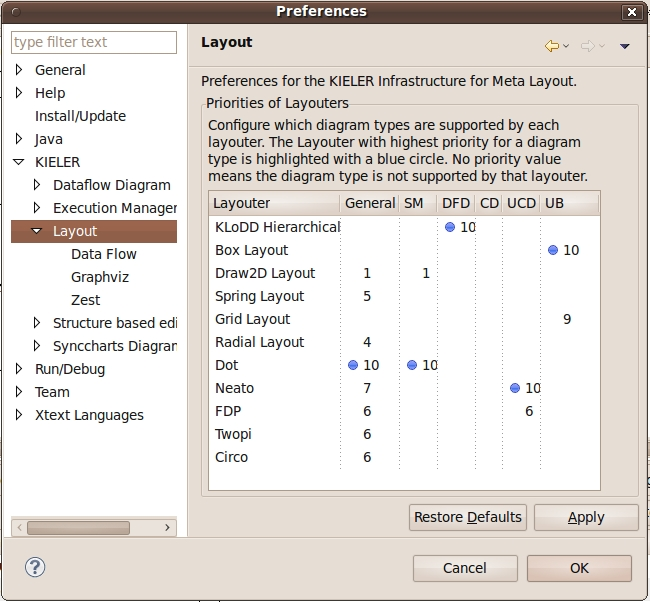
\includegraphics[scale=.5]{MSPLayoutPreferencePage.jpg}
  \caption[Layout Preference Page by Miro Sp\"onemann]%
  {Layout Preference Page by Miro Sp\"onemann\protect\footnotemark}
  \label{fig:MSPLayoutPreferencePage}
\end{figure}

Then we will construct another page for managing the different schedules
and their editors. For that we will adapt the LayoutPreferencePage by Miro Sp\"onemann
as seen in Figure \ref{fig:MSPLayoutPreferencePage} where we will just replace the 
layouts with the list of registered schedules.

In order to sort the schedules that match the currently opened editor they will
need to have user defined priorities which can be easily set up with the table
shown above.

The last page will be used to allow the user to set up his own properties and give them
default values.

The values entered in those pages will be stored inside the Eclipse Preference
Store.

%\begin{itemize}
% \item eclipse preference page architecture
% \item plug into KIELER preference page tree, create series of elements to
% configure item that are now only configurable through KiemView 
% \item use eclipse preference store to save values
% \item multiple pages for different aspects, user friendly, easier to maintain
%\end{itemize}

\section{Easier Configuration loading}
\label{section:ConfConceptsEasyLoading}
For easier configuration loading we will add two ComboBoxes to the existing
tool bar inside the \ac{KIEM} view.

One of them will display the list of recently used schedules the other one the
list of schedules that work for the currently active editor.

As soon as the user opens a new execution file through the normal workspace
view we will be notified of that event by the \ac{KIEM}. We will then create a new
schedule and store the path to the execution file in it along with the editor
that was opened at the time that the schedule was created. The new schedule will
also be added to the list of recently used schedules that we maintain through the 
use of the Eclipse preference store.

When the user selects one of the previously saved schedules in one of the
ComboBoxes we will retrieve the saved path and offer it to the KiemPlugin to
load it in the hopes that the execution file is still in the same location and
wasn't deleted, renamed or moved by the user.

% \begin{itemize}
%  \item keep a list of recently opened schedules in the preference store
%  \item allow access to that list through either menus or the KIEM itself
%  \item pass the saved path to KIEMPlugin to load it
%  \item store a list of editors that work for each .execution file together with their path
%  \item determine which editor is open and find matching files
% \end{itemize}